\documentclass[12pt,a4paper]{article}

\usepackage[fleqn]{amsmath} % This package with the fleqn option aligns equations to the left
\setlength{\mathindent}{0pt} % Set indentation from the left margin

\usepackage{amssymb} % Required for math symbols
\usepackage{graphicx} % Required for inserting images
\usepackage{geometry}

\usepackage[backend=biber, style=authoryear, citestyle=authoryear]{biblatex}
\addbibresource{references.bib}

\geometry{a4paper, margin=1in}

{
\title{
    
\includegraphics[width=0.4\textwidth]{/Users/mlnick/documents/images/tsukuba-logo.png} \\
    \textbf{Systems and Control} \\
    \vspace{3mm}    
    Report 4 on the Individual Task
}

\author{Mamanchuk Mykola, SID.202420671}
\date{\today}
}

\usepackage{listings}
\usepackage{color}

\definecolor{codegreen}{rgb}{0,0.6,0}
\definecolor{codegray}{rgb}{0.5,0.5,0.5}
\definecolor{codepurple}{rgb}{0.58,0,0.82}
\definecolor{backcolour}{rgb}{0.99,0.99,0.99}

\lstdefinestyle{mystyle}{
    backgroundcolor=\color{backcolour},   
    commentstyle=\color{codegreen},
    keywordstyle=\color{magenta},
    numberstyle=\tiny\color{codegray},
    stringstyle=\color{codepurple},
    basicstyle=\ttfamily\footnotesize,
    breakatwhitespace=false,         
    breaklines=true,                 
    captionpos=b,                    
    keepspaces=true,                 
    numbers=left,                    
    numbersep=5pt,                  
    showspaces=false,                
    showstringspaces=false,
    showtabs=false,                  
    tabsize=2
}
\lstset{style=mystyle}

\begin{document}

\maketitle

\section{Analysis of Two Phase-Coupled Oscillators}

\begin{center}
    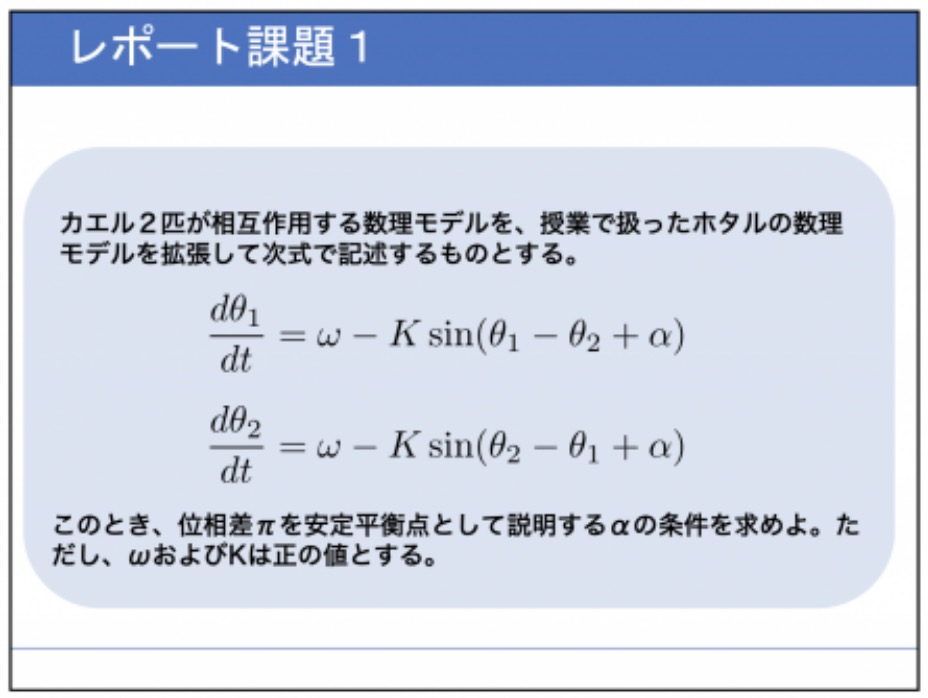
\includegraphics[width=0.6\textwidth]{materials/task0.jpeg}
\end{center}

\subsection{Problem Formulation}
The system consists of two oscillators (frogs) whose phase dynamics are influenced by a sinusoidal coupling and an additional phase shift. The differential equations governing their behavior are:
\begin{align}
    \frac{d\theta_1}{dt} &= \omega - K \sin(\theta_1 - \theta_2 + \alpha), \\
    \frac{d\theta_2}{dt} &= \omega - K \sin(\theta_2 - \theta_1 + \alpha).
\end{align}

\subsection{Phase Difference and System Dynamics}
Defining the phase difference \(\phi = \theta_1 - \theta_2\), we calculate the derivative of \(\phi\) with respect to time. We then subtract the derivative of \(\theta_2\) from \(\theta_1\) to find \(\frac{d\phi}{dt}\):
\begin{align}
    \frac{d\phi}{dt} &= \frac{d\theta_1}{dt} - \frac{d\theta_2}{dt} = \left(\omega - K \sin(\theta_1 - \theta_2 + \alpha)\right) - \left(\omega - K \sin(\theta_2 - \theta_1 + \alpha)\right).
\end{align}

Using the trigonometric identity for \(\sin(-x) = -\sin(x)\), the equation simplifies to:
\begin{align}
    \frac{d\phi}{dt} &= -K \sin(\theta_1 - \theta_2 + \alpha) + K \sin(\theta_2 - \theta_1 + \alpha).
\end{align}

Applying the sum-to-product identities for sine:
\[
\sin(a) - \sin(b) = 2 \cos\left(\frac{a + b}{2}\right) \sin\left(\frac{a - b}{2}\right)
\]
with \(a = \theta_2 - \theta_1 + \alpha\) and \(b = \theta_1 - \theta_2 + \alpha\), we derive:
\begin{align}
    \frac{d\phi}{dt} &= 2K \cos(\alpha) \sin(\theta_2 - \theta_1) = 2K \cos(\alpha) \sin(-\phi) = -2K \cos(\alpha) \sin(\phi).
\end{align}

This shows how the phase difference's rate of change depends on both the sine of the phase difference and the cosine of the additional phase shift \(\alpha\).

\subsection{Equilibrium and Stability Analysis}
\subsubsection{Equilibrium Points}
To find the equilibrium points, we set the rate of change of the phase difference to zero:
\begin{equation}
    -2K \cos(\alpha) \sin(\phi) = 0
\end{equation}
This condition implies that:
\begin{itemize}
    \item \(\sin(\phi) = 0\) leading to \(\phi = n\pi\), where \(n\) is an integer, suggesting potential equilibrium points at \(\phi = 0, \pi, 2\pi, \ldots\).
    \item \(\cos(\alpha) = 0\) would make the derivative zero regardless of \(\phi\), but this is not considered further without additional context or constraints on \(\alpha\).
\end{itemize}

\subsubsection{Stability Analysis}
For stability analysis, we particularly consider small perturbations around \(\phi = \pi\). Let \(\phi = \pi + \epsilon\) where \(\epsilon\) is a small perturbation:
\begin{equation}
    \sin(\phi) \approx \sin(\pi + \epsilon) = -\epsilon
\end{equation}
The linearized form of the differential equation becomes:
\begin{equation}
    \frac{d\epsilon}{dt} = 2K \cos(\alpha) \epsilon
\end{equation}
To ensure stability, the coefficient of \(\epsilon\) in the linearized equation must be negative, implying:
\begin{equation}
    K \cos(\alpha) < 0
\end{equation}
Given \(K > 0\) (assuming the coupling strength is positive), this requires:
\begin{equation}
    \cos(\alpha) < 0
\end{equation}
Hence, \(\alpha\) must lie in the range \(\frac{\pi}{2} < \alpha < \frac{3\pi}{2}\) for the equilibrium at \(\phi = \pi\) to be stable.

\subsection{Conclusion 1}
The analysis reveals that for stable anti-phase synchronization (\(\phi = \pi\)) between the two oscillators, the phase shift \(\alpha\) must ensure that \(\cos(\alpha)\) is negative. This condition is met when \(\alpha\) is in the second or third quadrant of the unit circle, specifically within the range \(\frac{\pi}{2} < \alpha < \frac{3\pi}{2}\). This analysis provides insight into how intrinsic phase shifts between oscillators influence their collective dynamics and the conditions necessary for stabilizing their anti-phase state.

\subsection{Symmetric Interchangeability of Phase Differences}
In the given model, where the phase dynamics between two coupled oscillators are described, an assumption can be introduced that the phase difference \(\theta_1 - \theta_2\) and its inverse \(\theta_2 - \theta_1\) are symmetrically interchangeable. This assumption allows us to simplify the analysis and focus on the inherent symmetry in the interaction dynamics.

\subsubsection{Model Formulation with Symmetric Interchangeability}
Given the differential equations:
\begin{align}
    \frac{d\theta_1}{dt} &= \omega - K \sin(\theta_1 - \theta_2 + \alpha), \\
    \frac{d\theta_2}{dt} &= \omega - K \sin(\theta_2 - \theta_1 + \alpha).
\end{align}
Assuming symmetry, we consider \(\theta_1 - \theta_2\) and \(\theta_2 - \theta_1\) to be functionally equivalent in their contribution to the dynamics, only differing by a sign and a phase shift. This leads us to analyze the phase difference \(\phi = \theta_1 - \theta_2\) with the understanding that the behaviors for \(\phi\) and \(-\phi\) are mirrored.

\subsubsection{Implications of Symmetry}
With symmetric interchangeability, the differential for the phase difference, \(\frac{d\phi}{dt}\), can be expressed symmetrically as:
\[
\frac{d\phi}{dt} = -2K \sin(\phi + \alpha).
\]
This form implies that the system's response to the phase difference \(\phi\) and its negative \(-\phi\) will have identical magnitudes but opposite directions, reflecting the symmetrical nature of their interactions.

\subsubsection{Stability Analysis Under Symmetric Conditions}
The stability of the system can be analyzed by setting \(\frac{d\phi}{dt} = 0\), which yields:
\[
\sin(\phi + \alpha) = 0.
\]
Solving for \(\phi\) gives equilibrium points at \(\phi + \alpha = n\pi\), where \(n\) is an integer. To ensure these points are stable:
\[
\cos(\phi + \alpha) < 0 \quad \text{for stability around these points.}
\]
The linear stability can further be examined by considering small perturbations around these equilibrium points and analyzing the resulting behavior based on the derived conditions.

\subsubsection{Analysis of Small Perturbations and Stability}
Next, we consider small perturbations around \(\phi + \alpha = n\pi\). Let \(\epsilon\) be a small perturbation such that \(\phi = n\pi - \alpha + \epsilon\). Substituting into the sinusoidal function, we use the linear approximation:
\[
\sin(\phi + \alpha) \approx \sin(n\pi + \epsilon) = (-1)^n \epsilon.
\]
The differential equation for \(\phi\) then becomes:
\[
\frac{d\phi}{dt} = -2K \sin(\phi + \alpha) \approx -2K (-1)^n \epsilon = (-1)^{n+1} 2K \epsilon.
\]
The sign of the coefficient of \(\epsilon\) in this linearized equation determines the stability:
\begin{itemize}
    \item If \((-1)^{n+1} 2K > 0\), the equilibrium point is unstable because perturbations grow exponentially.
    \item If \((-1)^{n+1} 2K < 0\), the equilibrium point is stable because perturbations decay exponentially.
\end{itemize}
This implies that for stability, \(n\) must be such that \((-1)^{n+1} 2K\) is negative. Specifically:
\begin{itemize}
    \item For even \(n\), the term \((-1)^{n+1}\) becomes \(-1\) and the condition for stability is \(K > 0\).
    \item For odd \(n\), the term \((-1)^{n+1}\) becomes \(1\) and the condition for stability is \(K < 0\), which contradicts the positive nature of \(K\), indicating that these points are typically unstable.
\end{itemize}

\subsubsection{Conclusion 2}
This analysis highlights that only certain values of \(\phi\) relative to \(\alpha\) lead to stable equilibrium, specifically when \(n\) is even, which corresponds to \(\phi + \alpha = 2k\pi\) (where \(k\) is an integer). These conditions ensure that small deviations from the equilibrium will decay, leading to a stable system under minor perturbations. This approach underscores the importance of the phase shift \(\alpha\) and the system's intrinsic properties in determining the overall stability and behavior of the coupled oscillators.

\section{Model Formulation for Frog Interaction Dynamics}

\begin{center}
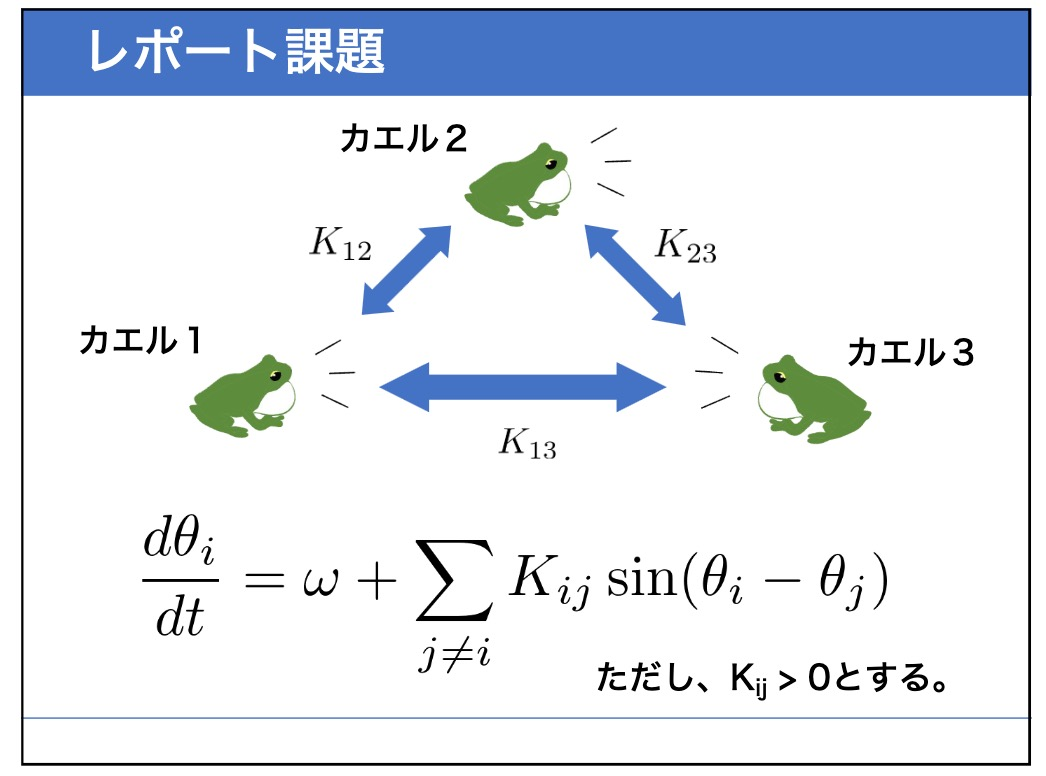
\includegraphics[width=0.6\textwidth]{materials/task1.jpeg}
\end{center}

\subsection{Model Formulation for Frog Interaction Dynamics}

\subsubsection{Task Description and Initial Conditions}
The task involves developing a mathematical model to describe the dynamic interactions between three frogs, labeled as Frog 1, Frog 2, and Frog 3. Each frog's croaking phase, denoted by $\theta_i$, is influenced by the others through sinusoidal coupling, represented by the coupling constants $K_{12}$, $K_{23}$, and $K_{13}$.

\subsubsection{Objective}
The objective is to formulate a set of differential equations capturing the phase dynamics of each frog, considering the sinusoidal nature of the interactions modulated by the coupling strengths.

\subsubsection{Mathematical Model Development}
The phase of croaking for each frog is described by a differential equation incorporating the natural frequency and the sinusoidal interactions from the other frogs:
\begin{align}
\frac{d\theta_1}{dt} &= \omega + K_{12} \sin(\theta_2 - \theta_1) + K_{13} \sin(\theta_3 - \theta_1), \\
\frac{d\theta_2}{dt} &= \omega + K_{12} \sin(\theta_1 - \theta_2) + K_{23} \sin(\theta_3 - \theta_2), \\
\frac{d\theta_3}{dt} &= \omega + K_{13} \sin(\theta_1 - \theta_3) + K_{23} \sin(\theta_2 - \theta_3).
\end{align}
Here, $\omega$ represents the natural croaking frequency assumed to be constant across all frogs, and $K_{ij}$ denotes the coupling constant from Frog $j$ to Frog $i$.

These equations set the foundation for analyzing the stability and synchronization behavior of the system in subsequent sections.

\subsection{Define Phase Differences}

\subsubsection{Objective}
To define the phase differences crucial for understanding the synchronization or anti-synchronization among the frogs.

\subsubsection{Definition of Phase Differences}
To analyze the interactions and synchronization dynamics more efficiently, we define the phase differences between the frogs as follows:
\begin{itemize}
    \item $\phi_{12} = \theta_1 - \theta_2$: This represents the phase difference between Frog 1 and Frog 2.
    \item $\phi_{23} = \theta_2 - \theta_3$: This represents the phase difference between Frog 2 and Frog 3.
    \item $\phi_{13} = \theta_1 - \theta_3$: This represents the phase difference between Frog 1 and Frog 3.
\end{itemize}
Note: $\phi_{13}$ is defined instead of $\phi_{31}$ to maintain consistency with the interaction directions initially provided.

\subsubsection{Differential Equations with Phase Differences}
Using the defined phase differences, the differential equations describing the system dynamics can be expressed as:
\begin{align}
\frac{d\theta_1}{dt} &= \omega + K_{12} \sin(-\phi_{12}) + K_{13} \sin(-\phi_{13}), \\
\frac{d\theta_2}{dt} &= \omega + K_{12} \sin(\phi_{12}) + K_{23} \sin(-\phi_{23}), \\
\frac{d\theta_3}{dt} &= \omega + K_{13} \sin(\phi_{13}) + K_{23} \sin(\phi_{23}).
\end{align}
Here, the sign of the sine function is adjusted based on the defined phase difference to correctly reflect the influence direction as stated in the coupling constants. $\omega$ represents the natural croaking frequency assumed to be constant across all frogs.

\subsection{Derive the System of Equations for Phase Differences}

\subsubsection{Objective}
The objective is to establish a system of differential equations that describe the interactions between the frogs solely in terms of the phase differences $\phi_{12}$, $\phi_{23}$, and $\phi_{13}$. This approach simplifies the analysis of synchronization dynamics within the group.

\subsubsection{Methodology}
Using the previously defined phase differences we rewrite the differential equations for each frog's phase to express these relations in terms of $\phi_{12}$, $\phi_{23}$, and $\phi_{13}$.

\subsubsection{Differential Equations with Phase Differences}
The initial system of differential equations is given by (4), (5), (6).
By subtracting these equations appropriately, we derive the system of equations for the phase differences:
\begin{align}
\frac{d\phi_{12}}{dt} &= \frac{d\theta_1}{dt} - \frac{d\theta_2}{dt} = -2K_{12} \sin(\phi_{12}) - K_{13} \sin(\phi_{13}) + K_{23} \sin(\phi_{23}), \\
\frac{d\phi_{23}}{dt} &= \frac{d\theta_2}{dt} - \frac{d\theta_3}{dt} = K_{12} \sin(\phi_{12}) - K_{13} \sin(\phi_{13}) - 2K_{23} \sin(\phi_{23}), \\
\frac{d\phi_{13}}{dt} &= \frac{d\theta_1}{dt} - \frac{d\theta_3}{dt} = -K_{12} \sin(\phi_{12}) - 2K_{13} \sin(\phi_{13}) + K_{23} \sin(\phi_{23}).
\end{align}

These equations allow us to focus on the dynamics of the phase differences between frogs, crucial for understanding their synchronization or anti-synchronization behavior.

\subsection{Linearization of the Differential Equations}

Now, we simplify the differential equations using linearization around an equilibrium point. This facilitates an analytical approach to studying the system's behavior near this point.

\subsubsection{Rationale for Choosing Zero Equilibrium}
Linearizing around the zero phase difference, \(\phi_{ij} = 0\), is particularly relevant for studying synchronization. This equilibrium point represents a state where all frogs are in perfect synchrony, with no phase difference between them. This state is not only straightforward to analyze mathematically but also significant biologically as it represents a potential stable configuration of the system. The small angle approximation, where \(\sin(x) \approx x\), is employed because it is valid for small values around zero and simplifies the sinusoidal interaction terms effectively.

\subsubsection{Linearization Process}
Using the small angle approximation, the sinusoidal functions in the differential equations are approximated as linear functions of the phase differences. This approximation transforms the nonlinear system into a linear one, which can be analyzed using standard methods in linear systems theory. The equations are linearized as follows:
\begin{align}
\frac{d\phi_{12}}{dt} &\approx -2K_{12} \phi_{12} - K_{13} \phi_{13} + K_{23} \phi_{23}, \\
\frac{d\phi_{23}}{dt} &\approx K_{12} \phi_{12} - K_{13} \phi_{13} - 2K_{23} \phi_{23}, \\
\frac{d\phi_{13}}{dt} &\approx -K_{12} \phi_{12} - 2K_{13} \phi_{13} + K_{23} \phi_{23}.
\end{align}

These linearized equations can now be assembled into a matrix form to analyze the stability of the system using eigenvalue analysis, which will be elaborated in the subsequent steps.

\subsubsection{Implications}
Linearization provides a means to evaluate the stability of the synchronization state under small perturbations. If the zero equilibrium is stable, any small deviation from synchronization will decay, suggesting robust synchrony among the frogs. Conversely, instability would imply that small disturbances could lead to significant desynchronization, highlighting sensitive dynamics within the system.

\subsection{Construction of the Jacobian Matrix}
Next, we formulate the Jacobian matrix from the linearized differential equations to analyze the local stability around the equilibrium point.

\subsubsection{Methodology}
\begin{itemize}
    \item First, determine the partial derivatives of each linearized differential equation with respect to each phase difference variable $\phi_{12}$, $\phi_{23}$, and $\phi_{13}$.
    \item Then, assemble these derivatives into the Jacobian matrix.
\end{itemize}

\subsubsection{Partial Derivatives}
The partial derivatives of the linearized equations are calculated as follows:
\begin{align}
\frac{\partial}{\partial \phi_{12}} \text{  of  } \frac{d\phi_{12}}{dt} &= -2K_{12}, \quad \frac{\partial}{\partial \phi_{23}} = K_{23}, \quad \frac{\partial}{\partial \phi_{13}} = -K_{13} \\
\frac{\partial}{\partial \phi_{12}} \text{  of  } \frac{d\phi_{23}}{dt} &= K_{12}, \quad \frac{\partial}{\partial \phi_{23}} = -2K_{23}, \quad \frac{\partial}{\partial \phi_{13}} = -K_{13} \\
\frac{\partial}{\partial \phi_{12}} \text{  of  } \frac{d\phi_{13}}{dt} &= -K_{12}, \quad \frac{\partial}{\partial \phi_{23}} = K_{23}, \quad \frac{\partial}{\partial \phi_{13}} = -2K_{13}
\end{align}

\subsubsection{Jacobian Matrix}
The Jacobian matrix $J$ is constructed as follows:
\[
J = \begin{bmatrix}
-2K_{12} & K_{23} & -K_{13} \\
K_{12} & -2K_{23} & -K_{13} \\
-K_{12} & K_{23} & -2K_{13}
\end{bmatrix}
\]

\subsection{Eigenvalue Analysis}

In this section, we calculate the eigenvalues of the Jacobian matrix to assess the stability of the equilibrium state where all phase differences are zero.

\subsubsection{Methodology}
Eigenvalues of the matrix are computed to determine the system's behavior near the equilibrium. Stability is inferred based on the nature of these eigenvalues:
\begin{itemize}
    \item Negative real parts indicate a stable equilibrium.
    \item Positive real parts indicate an unstable equilibrium.
    \item Purely imaginary eigenvalues suggest oscillatory behavior, requiring further analysis.
\end{itemize}

\subsubsection{Results of Eigenvalue Calculation}
The eigenvalues calculated from the Jacobian matrix \([[-2, 1, -1], [1, -2, -1], [-1, 1, -2]]\) are as follows:
\begin{itemize}
    \item $\lambda_1 = -1$
    \item $\lambda_2 = -2$
    \item $\lambda_3 = -3$
\end{itemize}
These eigenvalues are all negative, indicating that the equilibrium point is stable. This suggests that small perturbations around the equilibrium will decay exponentially, leading the system back to the state of synchronization.

\subsubsection{Conclusion}
The negative eigenvalues confirm that the system is stable at the zero phase difference equilibrium. This stability implies that the frogs' croaking will naturally synchronize under small deviations, demonstrating robustness in their synchronized state.


\subsection{Additional Thoughts}

\subsubsection{Supplementary Analysis: Asymmetric Conditions}
An alternative scenario was analyzed where \(\phi_{12} = \pi\), \(\phi_{23} = 0\), and \(\phi_{13} = \pi\). The linearization of the equations with these phase conditions, assuming small deviations around \(\pi\), resulted in a Jacobian matrix that produced positive eigenvalues. This indicates that the equilibrium under these conditions is unstable, leading to increased likelihood of desynchronization among the frogs if perturbed.

\subsubsection{Biological Implications}
From a biological perspective, the stability under symmetric conditions might suggest that the frogs have evolved mechanisms that favor synchronization, potentially as a survival or mating strategy. The instability in asymmetric conditions could indicate that precise alignment in phase differences is crucial for maintaining this synchronization, reflecting sensitivity to initial conditions in their natural behaviors.

\subsubsection{Conclusion}
These results underscore the importance of initial conditions in the dynamics of synchronized behaviors. Stability is only assured under symmetric conditions, while any deviation, particularly to a phase difference of \(\pi\), as implied in the task itself, leads to instability, suggesting that such a system requires careful alignment to maintain equilibrium.

\textbf{PS}: As excected, I watched a video on youtube of frogs croaking and was impressed at something I wasn't realising before studying syncronization phenomemon on such a simple model.  

\section{Studying a Conditionally Simplified Model}

\begin{center}
    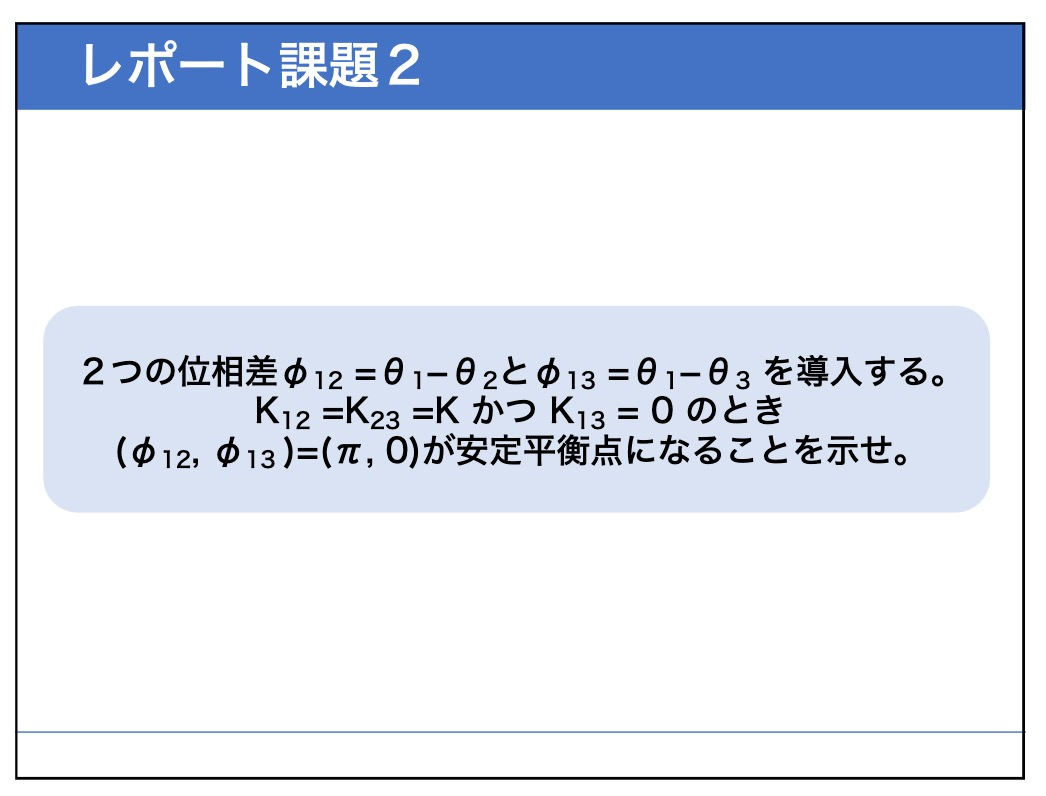
\includegraphics[width=0.6\textwidth]{materials/task2.jpeg}
\end{center}

\subsection{Formulation of the Problem and Differential Equations}

\subsubsection{Task Setup}
This task begins by defining the phase differences and constants for our system:
\begin{align*}
    \phi_{12} &= \theta_1 - \theta_2, \\
    \phi_{13} &= \theta_1 - \theta_3, \\
    K_{12} &= K_{23} = K, \quad K_{13} = 0.
\end{align*}
We are subsequently tasked with analyzing the system under the conditions where: \\ \((\phi_{12}, \phi_{13}) = (\pi, 0)\).

\subsubsection{System Dynamics}
Given the coupling constants and phase differences, the differential equations governing the dynamics of the system are:
\begin{align}
    \dot{\theta}_1 &= \omega + K \sin(\theta_1 - \theta_2) + 0 \cdot \sin(\theta_1 - \theta_3), \\
    \dot{\theta}_2 &= \omega + K \sin(\theta_2 - \theta_1) + K \sin(\theta_2 - \theta_3), \\
    \dot{\theta}_3 &= \omega + 0 \cdot \sin(\theta_3 - \theta_1) + K \sin(\theta_3 - \theta_2).
\end{align}

\subsubsection{Simplification under Given Conditions}
We assume small deviations \(\delta_{12}\), \(\delta_{23}\) around \(\pi\) and \(\delta_{13}\) around \(0\), defined as follows:
\begin{itemize}
    \item \(\phi_{12} = \pi + \delta_{12}\),
    \item \(\phi_{13} = \delta_{13}\),
    \item \(\phi_{23} = \pi + \delta_{23}\).
\end{itemize}
This leads to the following simplifications in the differential equations:
\begin{align}
    \dot{\theta}_1 &= \omega + K \sin(\pi + \delta_{12}) \approx \omega - K \delta_{12}, \\
    \dot{\theta}_2 &= \omega - K \sin(\pi + \delta_{12}) + K \sin(\pi + \delta_{23}) \approx \omega + K \delta_{12} - K \delta_{23}, \\
    \dot{\theta}_3 &= \omega + K \sin(\pi + \delta_{23}) \approx \omega + K \delta_{23}.
\end{align}
These linearized forms of the differential equations prepare us for subsequent analysis involving the construction of the Jacobian matrix and stability evaluation.

\subsection{Construction of the Jacobian Matrix}

Given the linearized differential equations, we construct the Jacobian matrix to analyze the stability of the system at the equilibrium point. The Jacobian matrix \(J\), derived from the partial derivatives of the system equations, is crucial for evaluating the local stability near the equilibrium.

The elements of the Jacobian matrix are determined as follows:
\begin{align*}
\frac{\partial \dot{\theta}_1}{\partial \delta_{12}} &= -K, & \frac{\partial \dot{\theta}_1}{\partial \delta_{13}} &= 0, & \frac{\partial \dot{\theta}_1}{\partial \delta_{23}} &= 0, \\
\frac{\partial \dot{\theta}_2}{\partial \delta_{12}} &= K, & \frac{\partial \dot{\theta}_2}{\partial \delta_{13}} &= 0, & \frac{\partial \dot{\theta}_2}{\partial \delta_{23}} &= -K, \\
\frac{\partial \dot{\theta}_3}{\partial \delta_{12}} &= 0, & \frac{\partial \dot{\theta}_3}{\partial \delta_{13}} &= 0, & \frac{\partial \dot{\theta}_3}{\partial \delta_{23}} &= K.
\end{align*}
The Jacobian matrix is then given by:
\[
J = \begin{bmatrix}
-K & 0 & 0 \\
K & 0 & -K \\
0 & 0 & K
\end{bmatrix}
\]
This matrix will be used in the subsequent eigenvalue analysis to determine the stability of the equilibrium.

\subsection{Eigenvalue Analysis and Conclusion}

\subsubsection{Eigenvalue Calculation}
Upon computing the eigenvalues of the Jacobian matrix, we find the eigenvalues to be \(\lambda = -1\), \(\lambda = 1\), and \(\lambda = 0\). The presence of these eigenvalues suggests diverse dynamical behaviors:

\begin{itemize}
    \item The eigenvalue \(\lambda = -1\) suggests damping or decay in one aspect of the system, leading to stabilization in that specific mode.
    \item The eigenvalue \(\lambda = 1\) indicates exponential growth in another mode, signifying instability.
    \item The eigenvalue \(\lambda = 0\) reflects the absence of dynamics (neither growth nor decay) along a particular direction, typically due to the lack of coupling in the system (\(K_{13} = 0\)).
\end{itemize}

\subsubsection{Interpretation and Conclusion}
The analysis of these eigenvalues reveals that the system does not settle into a stable equilibrium due to the positive eigenvalue, which drives the system towards instability. This characteristic is crucial for understanding the behavior under small perturbations and adjusting the system parameters to achieve desired control objectives or to avoid undesirable oscillations.

Furthermore, the system exhibits a neutral stability along one dimension, suggesting a potential line of constant solutions or undamped behavior depending on initial conditions and external inputs. This is particularly important in control systems where certain states might need to be maintained without convergence or divergence.

\subsubsection{Supplementary Analysis}
Given the asymmetry in the system setup (\(K_{13} = 0\)), and the resulting eigenvalue spectrum, it is evident that to achieve stability, modifications in the system's structural parameters or feedback mechanisms may be necessary. This underscores the sensitivity of the system's stability to its coupling coefficients and highlights areas for potential adjustment in design or operational protocols.



\setlength{\fboxsep}{0pt} % Removes padding around the image
\setlength{\fboxrule}{0.5pt} % Sets the thickness of the border

\section*{References}
\begin{enumerate}
    \item \textbf{Mamanchuk N., University of Tsukuba}, Github, \today. Available online: \url{https://github.com/RIFLE}
    % \item \textbf{Company}, Name of Work, year. Available online: \url{https://...} [Accessed: yyyy-mm-dd]
\end{enumerate}

\end{document}
›